\chapter{INTRODUÇÃO} \label{chap_introducao}

De acordo com a lei de Moore \cite{Intel}, o número de transistores em um circuito integrado dobra a cada dois anos. A princípio, a lei de Moore não passava de uma observação, porém com o tempo tornou-se um objetivo para a indústria eletrônica, como pode ser observado na Figura \ref{fig:lei_de_moore}:

\begin{figure}[H]
\centering
\caption{Lei de Moore.}
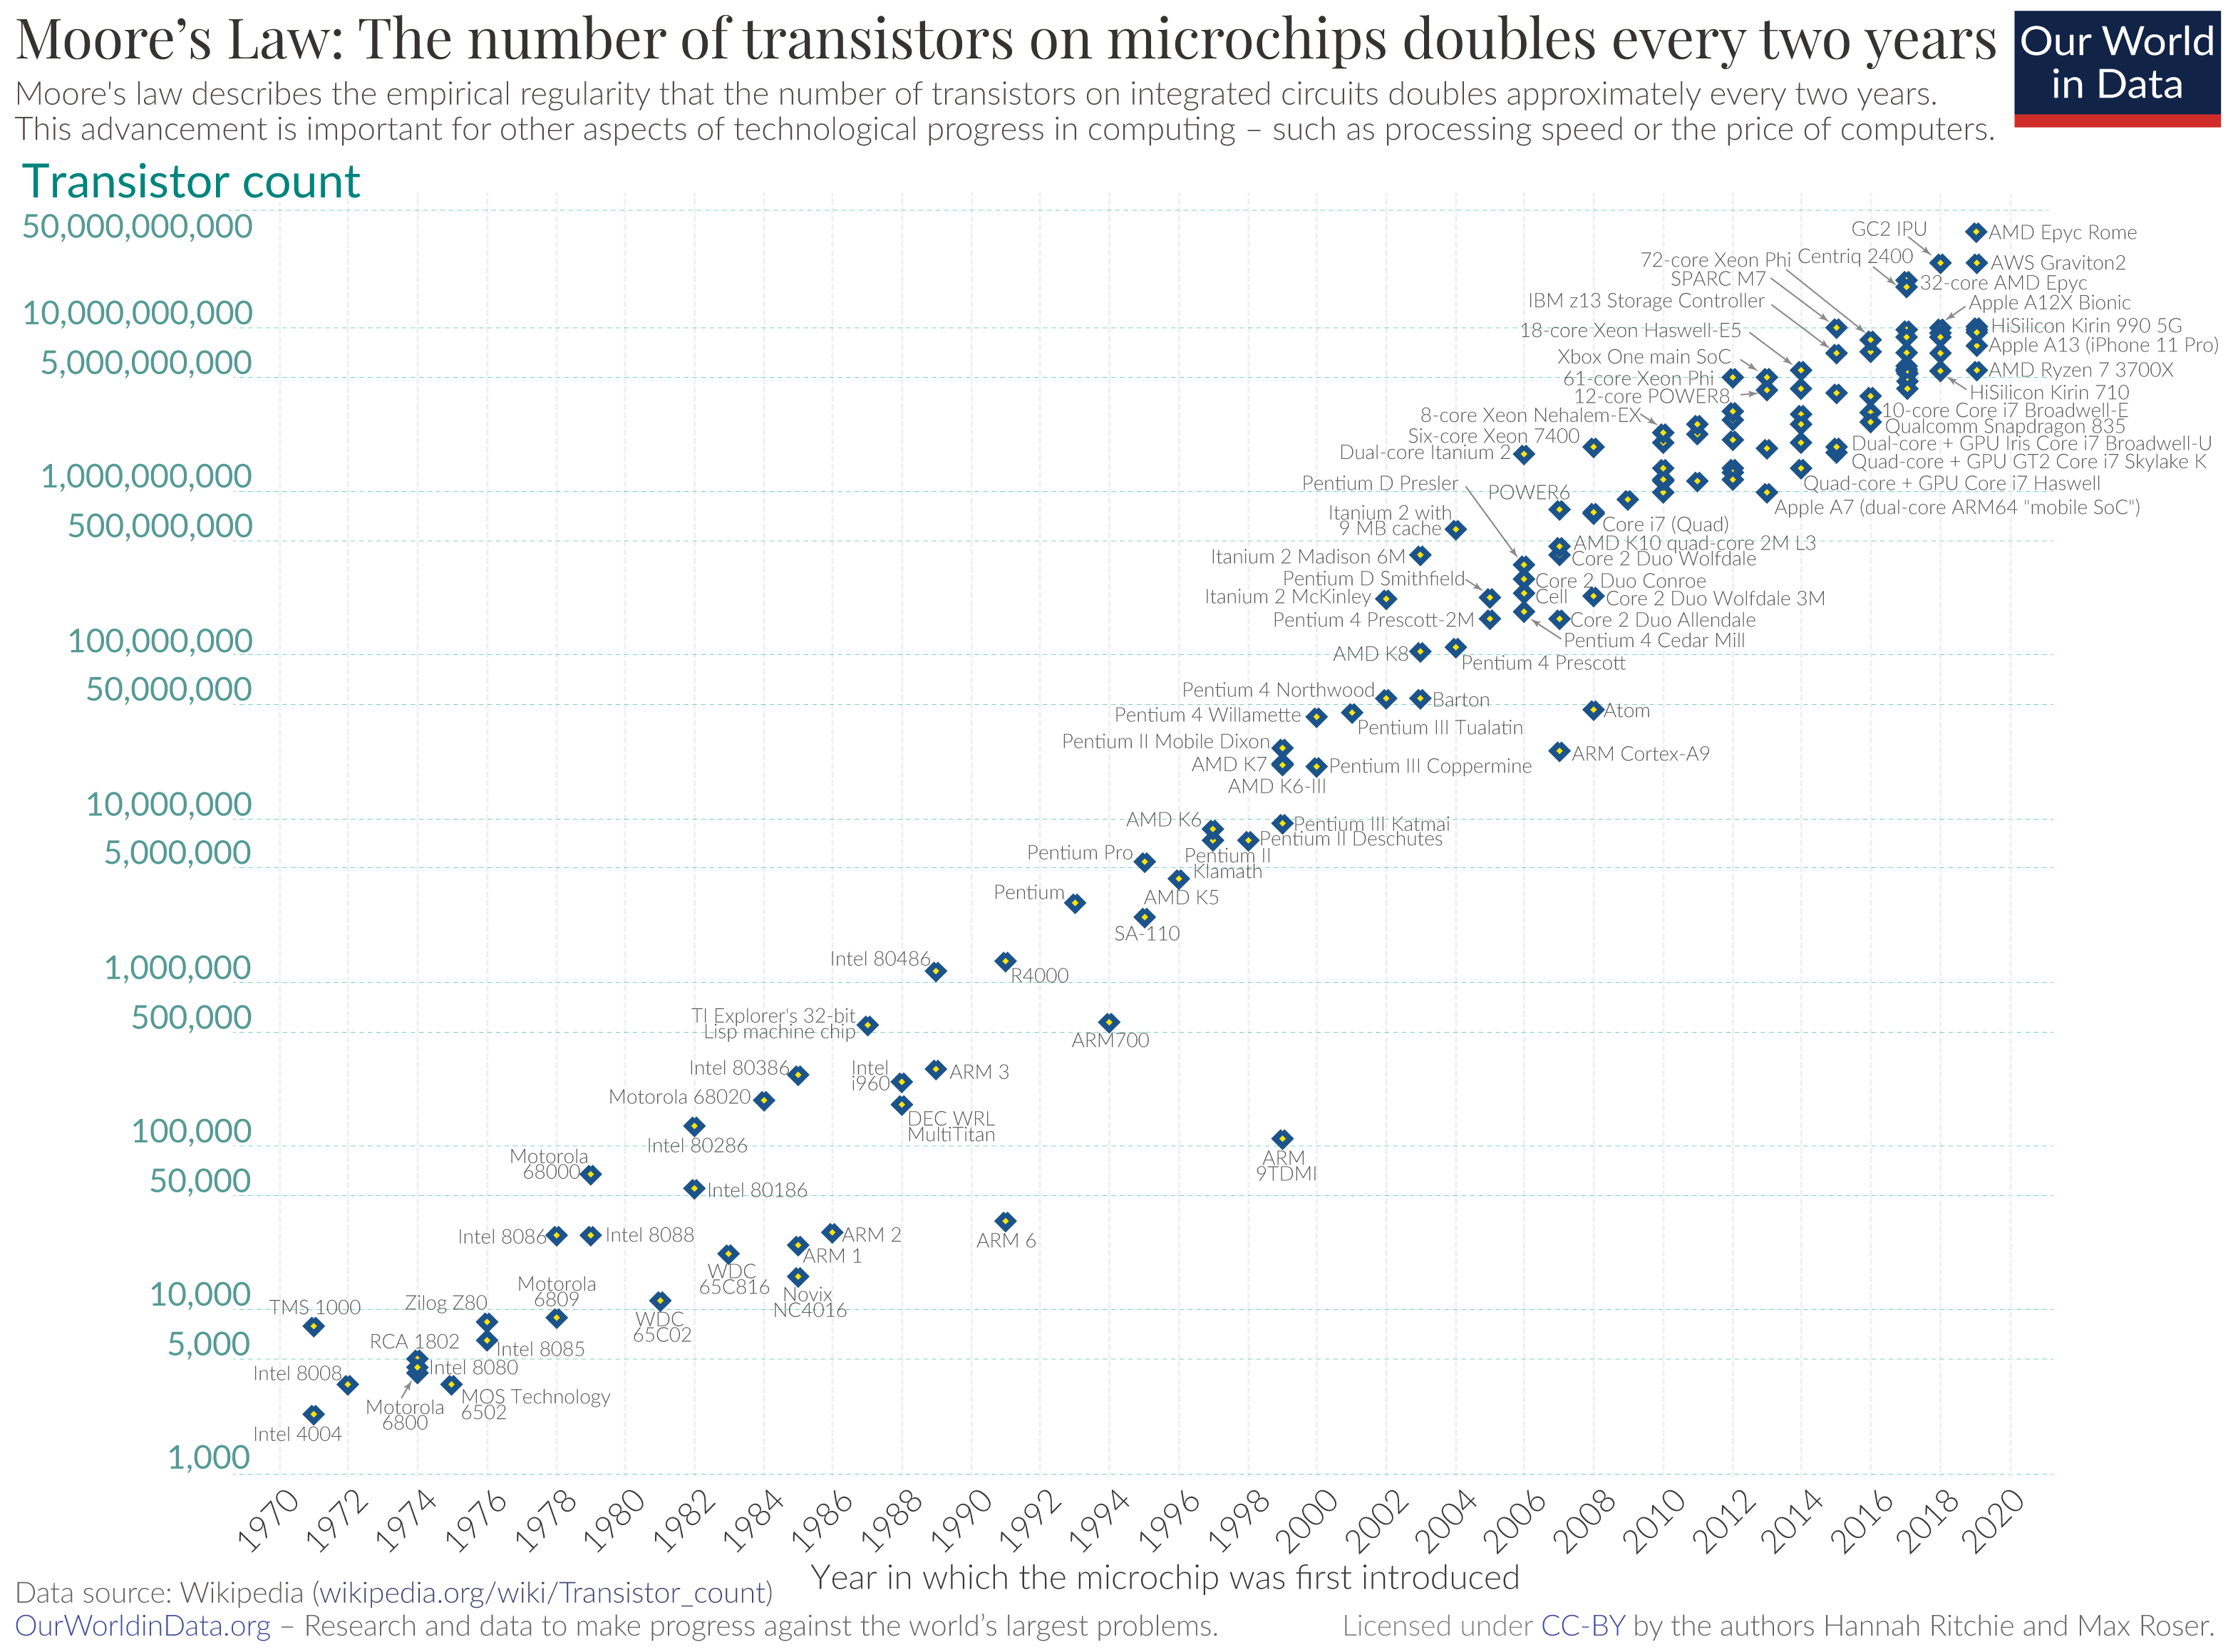
\includegraphics[scale=0.15]{imagens/Moores_Law.png}
\smallcaption{Fonte: Our World in Data.}
\label{fig:lei_de_moore}
\end{figure}

Com a produção e avanços crescentes de microchips e processadores, estamos chegando ao tamanho físico mínimo possível para um transistor e, com isto, o limite do poder de processamento de computadores clássicos pode estar se aproximando \cite{Nielsen}. Porém, a tendência é que a complexidade dos problemas computacionais continue a crescer; portanto, pode ser necessário recorrer a uma ferramenta como os computadores quânticos, que podem apresentar uma vantagem na solução de certos problemas considerados difíceis na computação clássica \cite{Mermin2007QComputerScience, Wong2022IntroductionClassicalQuantum}. 

Diferentemente dos computadores clássicos, os computadores quânticos são máquinas que fazem uso de propriedades da mecânica quântica para realizar suas operações \cite{Wong2022IntroductionClassicalQuantum}. Enquanto os computadores clássicos codificam e processam informações armazenadas em bits, os quânticos fazem essa codificação em qubits (bits quânticos), que permitem estados que correspondem a superposições entre os estados clássicos 0 e 1 \cite{Nielsen}. No entanto, as máquinas quânticas atuais ainda estão sujeitas a limitações e desafios significativos, que afetam sua capacidade de realizar tarefas de aprendizado de máquina de maneira eficiente.

Uma das principais limitações dos computadores quânticos atuais é o ruído. Os qubits são suscetíveis a erros causados por diversas fontes de ruído, desde raios cósmicos até a interação com os qubits vizinhos, passando pelo ruído térmico, eletrônico e eletromagnético \cite{Nielsen}. Esses erros podem levar a resultados incorretos e afetar a precisão dos cálculos realizados pelo computador quântico. O ruído é uma preocupação significativa em sistemas quânticos devido à sensibilidade dos qubits e à necessidade de manter a coerência quântica durante as operações.

Outra limitação dos computadores quânticos atuais é a falta de padronização e estabilidade. Diferentes arquiteturas e tecnologias são usadas na implementação de computadores quânticos, e não há um padrão único amplamente adotado. Isso torna difícil a reprodução de resultados em diferentes máquinas quânticas e dificulta a comparação de desempenho entre elas. Além disso, as tecnologias quânticas estão em constante evolução, e novas abordagens estão sendo exploradas, o que dificulta a estabilidade e confiabilidade dos sistemas quânticos atuais.

Essas limitações dos computadores quânticos atuais têm implicações significativas no uso dessas máquinas para tarefas de aprendizado de máquina. Algoritmos de aprendizado de máquina, como os utilizados na classificação de dados, dependem da precisão e da capacidade de processamento eficiente para obter resultados confiáveis. O ruído e a falta de padronização dos computadores quânticos podem afetar negativamente o desempenho desses algoritmos, tornando-os menos eficazes do que suas contrapartes clássicas.

Neste cenário, existem várias formas de classificação de dados em computadores quânticos que fazem uso de modelos de aprendizado de máquina supervisionados, dentre eles temos: \textit{quantum support vector machines} (QSVM) \cite{Rebentrost2014QSVM}, \textit{quantum principal component analysis} (qPCA) \cite{Lloyd2014qPCA}, \textit{quantum neural networks} (QNNs) \cite{Abhijith2022QuantumAlgorithm} entre outros. Todavia, este trabalho focará no classificador quântico variacional \cite{Havlicek2019qSupervisedLearning}, construído sobre a codificação no espaço de características quântico.

\section{Objetivo} \label{sec1}

Neste trabalho, busca-se investigar o desempenho atual de um computador quântico na tarefa de classificação de dados da base de dados Iris, comparando-o com um classificador clássico. A motivação por trás desse estudo é avaliar a capacidade do computador quântico real em relação a um problema de aprendizado de máquina, especificamente na área de classificação de dados.

Para isso, utiliza-se um método de aprendizado de máquina supervisionado, a máquina de vetores de suporte quântica, adaptada para ser executada em um computador quântico. A escolha da base de dados Iris como caso de estudo se deve à sua ampla utilização na comunidade científica como \textit{benchmark} para algoritmos de classificação.

Ao realizar essa comparação entre o classificador clássico e o computador quântico real, espera-se obter \textit{insights} sobre o atual desempenho dos computadores quânticos em tarefas de classificação de dados e identificar suas limitações. Essa análise contribuirá para o avanço da computação quântica e do campo de aprendizado de máquina, fornecendo informações importantes sobre as possibilidades e desafios envolvidos na aplicação de métodos quânticos nesse domínio.

Assim, este trabalho visa fornecer uma contribuição para a compreensão do estado atual da computação quântica em relação ao aprendizado de máquina e estabelecer uma base para futuras pesquisas e desenvolvimentos nessa área em constante evolução.

Em suma, será aplicado um classificador quântico variacional \cite{Havlicek2019qSupervisedLearning} para classificar o conjunto de dados Íris. O classificador será construído a partir de circuitos quânticos para codificação de informações clássicas em estados quânticos (\ref{Encoding}) e para aprendizagem (\ref{ansatz}). O circuito para aprendizagem tem topologia definida previamente e possui um conjunto de portas quânticas parametrizadas. O treinamento consiste em aprender os parâmetros das portas quânticas que otimizam a função de custo escolhida.

\section{Estrutura do Trabalho} \label{sec2}

O trabalho é dividido da seguinte maneira: Capítulo~\ref{chap_trabalhos_relacionados} contém os trabalhos relacionados, com o objetivo de apresentar o cenário atual da área. Capítulo~\ref{chap:conceitos} detalha todos os conceitos de física quântica utilizados. Capítulo~\ref{chap_metodologia} mostra a metodologia utilizada, ou seja, linguagem de programação, técnicas e etapas. Capítulo~\ref{chap_resultados} trata os resultados do projeto. Por fim, o Capítulo~\ref{chap_conclusao} discorre sobre as conclusões obtidas no desenvolvimento do trabalho.